%\documentclass[journal]{IEEEtran}
\documentclass[letterpaper,10pt,conference]{ieeeconf}

\IEEEoverridecommandlockouts                              % This command is only
                                                          % needed if you want to
                                                          % use the \thanks command
\overrideIEEEmargins
% See the \addtolength command later in the file to balance the column lengths
% on the last page of the document

\usepackage{amsmath,amssymb}
\usepackage{graphicx}                    % For pdf, bitmapped graphics files
\usepackage[usenames,dvipsnames]{xcolor} % For font in color
\usepackage{eurosym}                     % For writing sybmol for euro
\usepackage{siunitx}                     % For writing SI units
%\usepackage{subfigure}                   % For subfigures
%\usepackage{multirow}                    % Span table cells on multiple rows
%\usepackage{balance}                     % For ballancing the last page


% custom commands
\newcommand{\red}[1]{\textcolor{red}{#1}}  % we use red color for comments

\author{Nikolce Murgovski, Gabriel Rodrigues de Campos, Jonas Sj\"oberg
\thanks{The authors are with the Department of Signals and Systems, Chalmers University of Technology, Sweden. {\tt \{nikolce.murgovski, gabriel.campos, jonas.sjoberg\}@chalmers.se.}}%
\thanks{G. R. Campos is also with the DEIB, Politecnico di Milano, Italy. {\tt gabriel.rodriguesdecampos@polimi.it}}%
\thanks{The research leading to these results was supported by the grant AD14VARI02 - Progetto ERC BETTER CARS - Sottomisura B, the S2, SAFER, and by the European Commission Seventh Framework Programme under the project AdaptIVe, grant agreement number 610428.}% <-this % stops a space
}

\newlength \figwidth
\setlength \figwidth {\columnwidth}

\begin{document}
\title{Convex modeling of conflict resolution at traffic intersections}

\maketitle
\thispagestyle{empty}
\pagestyle{empty}


%%%%%%%%%%%%%%%%%%%%%%%%%%%%%%%%%%%%%%%%%%%%%%%%%%%%%%%%%%%%%%%%%%%%%%%%%%%%%%%%
\begin{abstract}
We study the problem of optimally controlling autonomous vehicles to safely cross an intersection. The problem is approached by solving an optimal control subproblem for all permutations of crossing sequences. For a chosen crossing sequence, we show that the subproblem of optimal longitudinal vehicle control, subject to collision avoidance constraints, can be formulated as a convex program. The proposed method transforms the problem from the original time domain to a space domain, and introduces a change of optimization variables by replacing vehicles' speed with its inverse. A case study is provided showing the effectiveness of the proposed method.
\end{abstract}


%%%%%%%%%%%%%%%%%%%%%%%%%%%%%%%%%%%%%%%%%%%%%%%%%%%%%%%%%%%%%%%%%%%%%%%%%%%%%%%%
\section{Introduction}


The development of Intelligent Transportation Systems (ITS) has enabled safer, smarter, and greener solutions  by leveraging advances in information technology to alleviate major problems in the current road traffic system~\cite{Behere2013}. Recent research has been focusing, among others, in prevention of accidents, reduction of greenhouse gas emissions and efficiency in terms of energy and infrastructure utilization.

A particular area of interest is efficient collision avoidance algorithms for traffic intersections \cite{Hafner2013,Doerzaph08a,Alexander11a}. In Europe,  intersections-related accidents are responsible for \SI{21}{\%} of traffic related deaths and \SI{43}{\%} of the non-fatal injuries \cite{Simon2009}. Similar numbers have been reported from the U.S. \cite{nhtsa2}. Due to the high risk of accidents, these scenarios are among the most regulated, with vehicles guided simultaneously by traffic lights, signs, road-markings and right-of-way rules. As a consequence, they often form bottlenecks and even when not causing congestion, existing coordination rules are inherently inefficient, enforcing unnecessary decelerations and stops and thereby wasting both fuel and time.

Cooperative ITS have the potential to improve traffic flow and safety near intersections, without relying on inefficient traffic lights or error-prone human control. Instead, vehicles equipped with communication devices, have to coordinate and agree on how to cross the intersection without collisions. Ideally, by exploiting their communication capabilities, the vehicles should be able to coordinate and achieve a quality of service requirement, such as the minimization of the aggregate fuel-consumption (e.g., by slowing down a light vehicle instead of a bus or a heavy truck).

This article focuses on cooperative conflict resolution techniques for fully autonomous vehicles.  Motivated by increasing levels of autonomy in passenger cars,  a lot of research efforts have been focusing on such scenarios. Using a rule-based approach, several works  approached the coordination problem based on the multi-agent systems paradigm \cite{dresner2004,dresner2005,dresner2008,kowshik2011}. Others, instead, used Model Predictive Control (MPC) coordination strategies ~\cite{kim2013mpc,kim2014mpc,Hult2015,Campos2013,Campos2014}. For instance, the authors of \cite{Hult2015} exploit the structure of a centralized, finite time optimal control problem, in order to propose an approximate solution, while \cite{Campos2013} considered a fully decentralized solution based on sub-optimal decision-making heuristics, using the concept of \emph{decision sequence}. This results were later extended in \cite{Campos2014}, where a low complexity receding horizon control framework is described. It is worth mentioning  that collision avoidance has also been approached from a safety verification point of view, where the driver is overridden in case  safety is compromised. Among others,   \cite{Hafner2013,Hafner2011,Hafner2011a} exploited hybrid systems theory and  \cite{Ahn2014,Bruni2013,Colombo2014,Colombo2012} a scheduling-based approach.

In this paper, we propose a novel approach where optimal control subproblems are solved for all permutations of crossing sequences. For such a set of solutions, our control algorithm provides optimal control trajectories for all vehicles, such that a quadratic cost function is minimized and collisions  avoided. We show that the optimal control subproblems can be formulated as a convex program where collision avoidance is enforced through spatial constraints rather than temporal conditions, as usually used in literature. To the best of our knowledge, such a convention, which may offer sound advantages when tackling complex scenarios, has not been proposed so far in literature. The contributions of this paper  are presented as follows: 1) modeling steps are provided that translate the linear time-dependent vehicle model into a linear position-dependent system; 2) variable changes are proposed  translating the time-dependent, non-convex, mixed-integer safety constraints into convex, position-dependent, linear constraints; 3) convex objective functions suitable for the position-dependent formulation are derived and analyzed.

The paper is organized as follows. Section \ref{sec:problemstatement} formulates the intersection crossing problem in time domain. Section \ref{sec:decoupled} decouples the optimization problem in scheduling and optimal control subproblem. In Section \ref{sec:convexmodeling} the optimal control subproblem is reformulated as a convex program, where collision avoidance is enforced through spatial constraints. Section \ref{sec:casestudy} provides a case study that shows the efficiency of the proposed method.  Section \ref{sec:conclusion} closes the  paper with final discussions and conclusions

%%%%%%%%%%%%%%%%%%%%%%%%%%%%%%%%%%%%%%%%%%%%%%%%%%%%%%%%%%%%%%%%%%%%%%%%%%%%%%%%
\section{Problem formulation} \label{sec:problemstatement}

\begin{figure}[t]
\centering
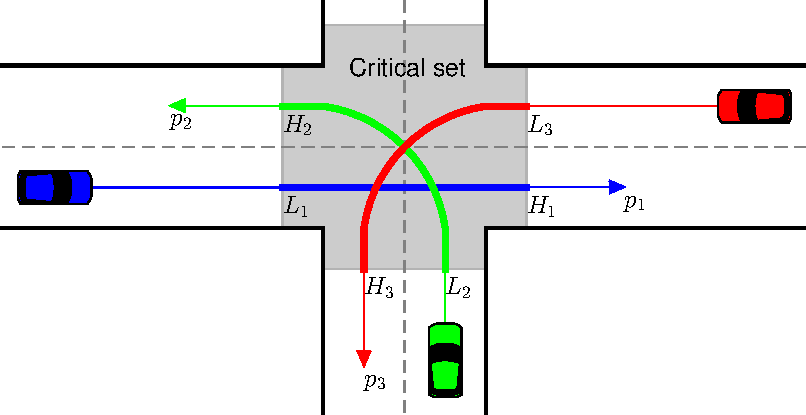
\includegraphics[width=\figwidth]{figures//intersection}
\caption{Illustration of a scenario where several autonomous vehicles approach an intersection, defined by a range of positions over pre-defined paths. Vehicles are approaching the intersection with a desired speed, where the control variable is the longitudinal acceleration.}
\label{fig:setup}
\end{figure}

Consider $N > 1$ autonomous vehicles approaching a traffic intersection as shown in Fig.~\ref{fig:setup}. For each vehicle $i$, we assume that:
 \begin{itemize}
 \item a path is given and is known;
 \item the assigned path is perfectly followed;
\item the acceleration along the path can be varied;
\item all vehicles have synchronized clocks and are located within a certain control radius centered at the intersection.
 \end{itemize}
The case where several vehicles approach the intersection on the same path, following each other, is not considered in this study.

%\textbf{Longitudinal dynamics.}
\subsubsection{Longitudinal dynamics}
Let \mbox{$\mathbf{x}_i(t)=[p_i(t) \; \dot p_i(t)]^T$} denote the state vector of vehicle $i$, consisting of the longitudinal position $p_i(t)$ and velocity $\dot p_i(t)$ along its path. A full measurement of the state $\mathbf{x}_i(t)$ is available at all times. Each vehicle is represented by a linear system
\begin{align}\label{eq:linsys1}
\mathbf{\dot x}_i(t)=A \mathbf{x}_i(t)+ B u_i(t), \; \forall i \in \mathcal{N},
\end{align}
with
\begin{align}
A=\left[\begin{array}{ccc} 0 & 1\\ 0 & 0 \end{array}\right], \; B=\left[\begin{array}{c} 0\\ 1 \end{array}\right],
\end{align}
where longitudinal acceleration is chosen as a control signal, i.e., $u_i(t)=\ddot p_i(t)$. The set of vehicle indices is \mbox{$\mathcal{N}=\{1,...,N \}$}.

As a part of the assigned driving task, each vehicle~$i$ is tracking a reference velocity $v_{ir}(t)$.

\subsubsection{State and control constraints} Each vehicle $i$ is subject to state and control constraints
\begin{align} \label{eq:statecstr}
&\mathbf{x}_i(t) \in [\mathbf{x}_{i\text{min}}(t), \mathbf{x}_{i\text{max}}(t)], \; \forall i \in \mathcal{N},\\
&u_i(t) \in [u_{i\text{min}}(t), u_{i\text{max}}(t)], \; \forall i \in \mathcal{N},
\end{align}
where the inequalities are imposed for all time instances \mbox{$t \in [0, t_{if}]$}. The final time $t_{if}$, when the vehicle reaches its final destination $p_{if}$, is free. 
\subsubsection{Critical set} For each vehicle $i \in \mathcal{N}$, let $\mathcal{C}_i$ denote the critical set,
\begin{align}
\mathcal{C}_i = \left\{ p_i(t)\in [0, p_{if}]\ |\ p_i(t)\in [L_i,H_i] \right\},
\end{align}
i.e., the set of all positions along the path where a collision is possible. Here, $L_i$ and $H_i$, with $L_i < H_i \leq p_{if}$, are bounds on the position along the path of vehicle $i$. Note that these parameters are dependent on the geometry of the workspace and are time-invariant.

\subsubsection{Occupancy interval} For each vehicle $i$, the occupancy interval
\begin{align}
\mathcal{G}_i(u_i(t))=\{t \in [0,t_{if}]\ | \ p_{i}(t) \in \mathcal{C}_i\},
\end{align}
defines the set of time instances when the vehicle $i$ resides within the critical set $\mathcal{C}_i$. Collision among vehicles is avoided if only one vehicle at a time resides within its respective critical set, i.e.,
\begin{align}
\mathcal{G}_i(u_i(t)) \cap  \mathcal{G}_j(u_j(t))=\emptyset, \; \forall i,j \in \mathcal{N}, \; j \neq i.
\end{align}

\subsubsection{Problem statement} The performance of the system is evaluated by a sum of cost functions
\begin{align}
\sum_{i=1}^N J_i(\mathbf{x}_i(t),u_i(t),\dot u_i(t), \mathbf{x}_i(t_{if}), t_{if}),
\end{align}
where the individual cost functions may differ for different vehicles. The functions $J_i(\cdot)$ may include penalties on final state, penalties for deviation from the reference velocity $v_{ir}(t)$, penalties for the control actions, penalties for changes in control actions (e.g., discomfort penalties associated to longitudinal jerk), or penalties for the total travel time, etc. Detailed implementation of these functions is deferred to Section \ref{sec:objective}.

We can now formulate the optimization problem as
{\allowdisplaybreaks
\begin{subequations} \label{eq:p1}
\begin{align}
&\min_{u_i(t), t_{if}} \sum_{i=1}^N J_i(\mathbf{x}_i(t),u_i(t),\dot u_i(t), \mathbf{x}_i(t_{if}), t_{if}) \label{eq:objective1}\\
&\text{subject to} \nonumber\\
&\mathbf{\dot x}_i(t)=A \mathbf{x}_i(t)+ B u_i(t), \; \forall i \in \mathcal{N}\\
&\mathbf{x}_i(t) \in [\mathbf{x}_{i\text{min}}(t), \mathbf{x}_{i\text{max}}(t)], \; \forall i \in \mathcal{N}\\
&u_i(t) \in [u_{i\text{min}}(t), u_{i\text{max}}(t)], \; \forall i \in \mathcal{N}\\
&\mathbf{x}_i(0)=\mathbf{x}_{i0}, \; \mathbf{x}_i(t_{if})=\mathbf{x}_{if}, \; \forall i \in \mathcal{N}\\
&\mathcal{G}_i(u_i(t)) \cap  \mathcal{G}_j(u_j(t))=\emptyset, \; \forall i,j \in \mathcal{N}, \; j \neq i, \label{eq:intersection1}
\end{align}
\end{subequations}}%
where the constraints are imposed element-wise, \mbox{$\forall t \in [0, t_{if}]$}. The initial and final state values are denoted by $\mathbf{x}_{i0}$ and $\mathbf{x}_{if}$, respectively, and satisfy \mbox{$\mathbf{x}_{i0} \in [\mathbf{x}_{i\text{min}}(0), \mathbf{x}_{i\text{max}}(0)]$}, \mbox{$\mathbf{x}_{if} \in [\mathbf{x}_{i\text{min}}(t_{if}), \mathbf{x}_{i\text{max}}(t_{if})]$}. Note that the actual final state values $\mathbf{x}_i(t_{if})$ are included both in the objective function and as a hard constraint in~\eqref{eq:p1}. This formulation is useful when only part of the states are constrained to a target state (e.g., the final position $p_{if}$), while other states (such as the final velocity) are only penalized in the objective. Optimization variables are the control trajectories $u_i(t)$ and the final times~$t_{if},\ \forall i \in \mathcal{N}$.

It is important to mention that the optimization problem~\eqref{eq:p1} is non-convex and mixed-integer. More precisely, the non-convexity arises from the mixed-integer constraint~(\ref{eq:intersection1}) enforcing safety, i.e., collision avoidance. This constraint is central in the formulation (\ref{eq:p1}), since it decides both the crossing order of the vehicles over the intersection, while at the same time preventing collisions by not allowing more than one vehicle to occupy their critical set at the same time. As such, the problem (\ref{eq:p1}) is difficult to solve. In order to tackle the complexity issue, the problem is decoupled in Section \ref{sec:decoupled} into two subproblems: 1) one that decides the crossing sequence, which we refer to as the scheduling problem, and 2) one that decides the control signals $u_i(t)$ and prevents collisions, which we refer to as the optimal control subproblem. Later, in Section \ref{sec:convexmodeling}, we provide our main contribution by proposing a computationally efficient method for solving the optimal control subproblem.

%%%%%%%%%%%%%%%%%%%%%%%%%%%%%%%%%%%%%%%%%%%%%%%%%%%%%%%%%%%%%%%%%%%%%%%%%%%%%%%%
\section{Decoupled scheduling/control formulation} \label{sec:decoupled}

One possible way to approach problem (\ref{eq:p1}) is by a nested optimization, where the optimal control subproblem is solved for all possible crossing sequences generated in an outer loop. The optimal solution is then obtained by selecting the crossing sequence that minimizes the objective (\ref{eq:objective1}). Therefore, for the optimal crossing sequence, the optimal control policies are those  minimizing objective (\ref{eq:objective1}) while avoiding collisions among vehicles.

\subsubsection{Crossing sequence} Let $\mathcal{O}\in\mathcal{N}^{M\times N}$ be a matrix with \mbox{$M=N!$} rows and $N$ columns, where each row contains a unique permutation of the elements in $\mathcal{N}$. Then, a crossing sequence $m$ is indicated as the $m$-th row in $\mathcal{O}$, while the index of the $n$-th vehicle in that crossing sequence is indicated by $\mathcal{O}_{m,n}$.

For a given crossing sequence $m$, the optimal control subproblem can be formulated as

{\allowdisplaybreaks
\begin{subequations} \label{eq:p2}
\begin{align}
&V_{m}(\cdot)=\min_{u_i(t), t_{if}} \sum_{i=1}^N J_i(\mathbf{x}_i(t),u_i(t),\dot u_i(t), \mathbf{x}_i(t_{if}), t_{if}) \nonumber\\
&\text{subject to} \nonumber\\
&\mathbf{\dot x}_i(t)=A \mathbf{x}_i(t)+ B u_i(t), \; \forall i \in \mathcal{N} \label{eq:linsys2}\\
&\mathbf{x}_i(t) \in [\mathbf{x}_{i\text{min}}(t), \mathbf{x}_{i\text{max}}(t)], \; \forall i \in \mathcal{N} \label{eq:statecstr2}\\
&u_i(t) \in [u_{i\text{min}}(t), u_{i\text{max}}(t)], \; \forall i \in \mathcal{N} \label{eq:controlcstr2}\\
&\mathbf{x}_i(0)=\mathbf{x}_{i0}, \; \mathbf{x}_i(t_{if})=\mathbf{x}_{if}, \; \forall i \in \mathcal{N}\\
\begin{split} \label{eq:intersection2}
&t_k \leq t_l, \; \forall t_k \in \mathcal{G}_{\mathcal{O}_{m,n}}(\cdot), \; \forall t_l \in \mathcal{G}_{\mathcal{O}_{m,n+1}}(\cdot)\\
&\hspace{13mm}n=1,...,N-1,
\end{split}
\end{align}
\end{subequations}}%
where collision avoidance is enforced by (\ref{eq:intersection2}), which states that the time when vehicle $k$ exits the critical set must be less than or equal to the time when the following vehicle $l$ in the sequence enters the critical set.

The solution to the original problem (\ref{eq:p1}) is then obtained by selecting the crossing sequence with minimum cost such that
\begin{align}
\min_{m}\; V_{m}(u_i^*(t), t_{if}^*), \;  m=1,...,M,
\end{align}
where the star superscript indicates the optimal solution obtained by solving the optimal control subproblem \eqref{eq:p2} for the crossing sequence $m$.

The difference between the control problem (\ref{eq:p2}) and the original formulation (\ref{eq:p1}) may seem subtle, as these formulations differ only at the constraints (\ref{eq:intersection2}) and (\ref{eq:intersection1}). However, the constraint (\ref{eq:intersection1}) requiring zero cardinality of occupancy intervals intersection, is transformed in (\ref{eq:intersection2}) into a simpler inequality constraint. However, problem (\ref{eq:p2}) is still not easy to solve, as there is no easy way to obtain the optimal entry/exit times satisfying the collision avoidance constraint (\ref{eq:intersection2}). A final transformation of problem (\ref{eq:p2}) will be provided in the following section, where the optimal control subproblem is reformulated as a convex program.

%%%%%%%%%%%%%%%%%%%%%%%%%%%%%%%%%%%%%%%%%%%%%%%%%%%%%%%%%%%%%%%%%%%%%%%%%%%%%%%%%
\section{Convex modeling of the control subproblem} \label{sec:convexmodeling}
In this section, the optimal control subproblem (\ref{eq:p2}) is reformulated as a convex program, given that cost functions $J_i(\cdot)$ are chosen to be convex. A central point in the proposed method is the collision avoidance constraint (\ref{eq:intersection2}), for which we propose an exact convex reformulation. The proposed convex modeling steps include sampling in distance, change of variables and linearization. 

%%%%%%%%%%%%%%%%%%%%%%%%%%%%%%%%%%%%%%%%%%%%%%%%%%%%%%%%%%%%%%%%%%%%%%%%%%%%%%%%%
\subsection{Sampling in distance and variable change} \label{sec:samplingdistance}

In order to reformulate (\ref{eq:intersection2}) as a convex constraint, two problem transformations are performed. First, the linear system (\ref{eq:linsys2}) is transformed via sampling in space, rather than time. Here, we use a shorthand notation $(\cdot)'$ to denote a derivative with respect to distance, i.e., $x'=d x/dp$. Second, we propose a variable change $z_i(t)=1/\dot p_i(t)$, which denotes the inverse of vehicle speed.

\subsubsection{Lethargy} The variable $z_i$, with unit seconds/meters, indicates the slowness or lack of energy of the system. In the rest of the paper we refer to $z_i$ as lethargy.

\subsubsection{Longitudinal dynamics} Let \mbox{$\mathbf{\tilde x}_i(p)=[t_i(p) \; z_i(p)]^T$} denote the state vector of vehicle $i$, when the system is sampled in the spatial coordinate $p$. Each vehicle is now represented by the linear system
\begin{equation}\label{model}
\mathbf{\tilde x'}_i(p)=A \mathbf{\tilde x}_i(p)+ B \tilde u_i(p), \; \forall i \in \mathcal{N},
\end{equation}
where spatial derivative of lethargy is chosen as the control signal, i.e., \mbox{$\tilde u_i(p)=z_i'(p)$}, and the matrices $A$ and $B$ are exactly as in (\ref{eq:linsys1}). Note that in this formulation the travel time of each vehicle $i$ becomes a state in the system. Starting from the basic definition of vehicle speed, $\dot p_i(t)=dp/dt$, it follows that the travel time of each vehicle is related to the lethargy by $t'_i(p)=z_i(p)$.

\subsubsection{Occupancy interval for a given crossing sequence} The safety constraint (\ref{eq:intersection2})  is now transformed into $N-1$ linear inequality constraints given by
\begin{align} \label{eq:intersection2_1}
\begin{split}
t_k(H_k) \leq t_l(L_l), \; k=\mathcal{O}_{m,n}, \; l&=\mathcal{O}_{m,n+1}, \\
n&=1,...,N-1,
\end{split}
\end{align}
where $k, l$ are indices of consecutive vehicles in a certain crossing sequence $m$. The constraints (\ref{eq:intersection2_1}) simply state that the time the vehicle $k$ exits the critical set must be less than or equal to the time the following vehicle $l$ enters the critical set.

\subsubsection{State and control constraints} Let $v_{i\text{min}}(t)$, $v_{i\text{max}}(t)$, $a_{i\text{min}}(t)$, $a_{i\text{max}}(t)$, with $0 < v_{i\text{min}}(t) \leq v_{i\text{max}}(t)$, \mbox{$a_{i\text{min}}(t) \leq 0$}, \mbox{$a_{i\text{max}}(t) \geq 0$}, $\forall t \in [0, t_{if}]$, denote the minimum and maximum speed and acceleration limits of the time-dependent formulation (\ref{eq:p1}). Then, the limits of the spatial state vector $\mathbf{\tilde x}_i(p)$ can be expressed as
\begin{align} \label{eq:statecstr2_1}
&\mathbf{\tilde x}_i(p) \in [\mathbf{\tilde x}_{i\text{min}}(p), \mathbf{\tilde x}_{i\text{max}}(p)], \; \forall i \in \mathcal{N},
\end{align}
where the inequalities are imposed for all sampling instances $p \in [0, p_{if}]$, and the limits are defined as
\begin{align}
\begin{split}\label{eq:statecstr2_2}
\mathbf{\tilde x}_{i\text{min}}(p)&=\left [\begin{array}{c} 0\\ 1/v_{i\text{max}}(p)\end{array}\right],\\
\mathbf{\tilde x}_{i\text{max}}(p)&=\left [\begin{array}{c} \int_0^{p_{if}} dp/v_{i\text{min}}(p)\\ 1/v_{i\text{min}}(p)\end{array}\right],
\end{split}
\end{align}
where the spatial speed limits $v_{i\text{min}}(p),\ v_{i\text{max}}(p)$ in (\ref{eq:statecstr2_2}) are an exact translation of the time-dependent state limits in (\ref{eq:statecstr}). Note that the total travel time of each vehicle is free, as we mentioned earlier, but it is upper bound by $\int_0^{p_{if}} 1/v_{i\text{min}}(p)dp$. The upper bound simply states that the longest travel time for each vehicle is the time needed to drive the distance $[0, p_{if}]$ with the minimum allowed speed $v_{i\text{min}}(p)$.

An exact translation of the acceleration limits into the spatial domain is given as
\begin{align} \label{eq:acclimit2_1}
&-\tilde u_i(p)\in z_i^3[a_{i\mathrm{min}}(p), a_{i\mathrm{max}}(p)],
\end{align}
which defines a non-convex set. The set (\ref{eq:acclimit2_1}) can be convexified by linearizing $z_i^3(p)$ about the reference speed $v_{ir}$, giving
\begin{align}
\begin{split} \label{eq:controlcstr2_2}
&\tilde u_{i\text{min}}(\cdot)=a_{i\text{max}}(p) \left(2 - 3 v_{ir}(p) z_i(p) \right)/v_{ir}^3(p)\\
&\tilde u_{i\text{max}}(\cdot)=a_{i\text{min}}(p) \left(2 - 3 v_{ir}(p) z_i(p) \right)/v_{ir}^3(p)
\end{split}\\
&\tilde u_i(p) \in [\tilde u_{i\text{min}}(p,z_i(p)), \tilde u_{i\text{max}}(p,z_i(p))], \; \forall i \in \mathcal{N}. \label{eq:controlcstr2_1}
\end{align}
This approximation underestimates the spatial domain maximum acceleration limit $a_{i\text{max}}(p)$ and overestimates the minimum acceleration limit $a_{i\text{min}}(p)$, thus ensuring that a solution obtained by enforcing (\ref{eq:controlcstr2_1}) is feasible to the original formulation as well. In normal driving conditions, when the vehicle is rarely operated at the acceleration limits, the linearization error will have small influence on the results. The error could be further decreased by re-linearizing about the optimal velocity trajectory, when the control problem is to be solved iteratively. This is a standard MPC practice \cite{mayne00}.

\subsubsection{Initial and final state constraints} Let \mbox{$\mathbf{x}_{i0}=[0 \; v_{i0}]^T$}, \mbox{$\mathbf{x}_{if}=[p_{if} \; v_{if}]^T$}, denote the initial and final state values of the time-dependent state vector $\mathbf{x}_i(t)$, where, without loss of generality, all vehicles are placed at zero initial position. Then, the initial and final values of the spatial state vector $\mathbf{\tilde x}_i(p)$ can be expressed as \mbox{$\mathbf{\tilde x}_{i0}=[0 \; 1/v_{i0}]^T$}, \mbox{$\mathbf{\tilde x}_{if}=[\text{free} \; 1/v_{if}]^T$}.

\subsubsection{Problem statement} We can now formulate the optimal control subproblem as
%{\allowdisplaybreaks
\begin{subequations} \label{eq:p3}
\begin{align}
&\min_{\tilde u_i(p)} \sum_{i=1}^N J_i(\mathbf{\tilde x}_i(p),\tilde u_i(p),\tilde u'_i(p), \mathbf{\tilde x}_i(p_{if}))\\
&\text{subject to} \nonumber\\
&\mathbf{\tilde x'}_i(p)=A \mathbf{\tilde x}_i(p)+ B \tilde u_i(p), \; \forall i \in \mathcal{N} \label{eq:linsys3}\\
&\mathbf{\tilde x}_i(p) \in [\mathbf{\tilde x}_{i\text{min}}(p), \mathbf{\tilde x}_{i\text{max}}(p)], \; \forall i \in \mathcal{N}\\
&\tilde u_i(p) \in [\tilde u_{i\text{min}}(p,z_i(p)), \tilde u_{i\text{max}}(p,z_i(p))], \; \forall i \in \mathcal{N}\\
&\mathbf{\tilde x}_i(0)=\mathbf{\tilde x}_{i0}, \; \mathbf{\tilde x}_i(p_{if})=\mathbf{\tilde x}_{if}, \; \forall i \in \mathcal{N}\\
\begin{split} \label{eq:intersection3}
&t_k(H_k) \leq t_l(L_l), \; k=\mathcal{O}_{m,n}, \; l=\mathcal{O}_{m,n+1}, \\
&\hspace{42.5mm}n=1,...,N-1,
\end{split}
\end{align}
\end{subequations}%}%
where, for a given crossing sequence $m$, the constraints (\ref{eq:linsys3})-(\ref{eq:intersection3}) are linear. Hence, if the cost functions $J_i(\cdot)$ are convex, the optimization problem (\ref{eq:p3}) is a convex program.

%%%%%%%%%%%%%%%%%%%%%%%%%%%%%%%%%%%%%%%%%%%%%%%%%%%%%%%%%%%%%%%%%%%%%%%%%%%%%%%%
\subsection{Convex cost functions} \label{sec:objective}
In this section we analyze cost functions that are commonly used in literature for the time-dependent problem formulation (\ref{eq:p1}), and we propose convex alternatives for the spatial problem formulation (\ref{eq:p3}).

\subsubsection{Velocity tracking} A commonly used cost function,  penalizing the deviation from a reference velocity, is given as
\begin{align} \label{eq:tracking1}
J_{i1}(\dot p_i(t))=w_{i1} \int_0^{t_{if}} (\dot p_i(t)-v_{ir}(t))^2 dt,
\end{align}
where $w_{i1}$ is a nonnegative penalty parameter that may have assigned a certain unit. An exact translation of (\ref{eq:tracking1}) into a spatial formulation with the usage of lethargy is %\begin{footnotesize}
\begin{align} \label{eq:trackingSOCP}
J_{i1}(z_i(p))=w_{i1} \int_0^{p_{if}} \left(\frac{1}{\sqrt{z_i(p)}}-v_{ir}(p)\sqrt{z_i(p)} \right)^2 dp,
\end{align}%\end{footnotesize}
which can be formulated as a convex second order cone function \cite{boyd04}. The resulting control problem (\ref{eq:p3}) is then a convex second order cone program (SOCP).

However, it is often desirable to formulate the problem as a convex quadratic program (QP), since QP solvers technology is more mature than SOCP, and QPs can be solved faster than SOCPs \cite{boyd04}. A quadratic cost alternative of (\ref{eq:trackingSOCP}) can be obtained by linearizing the term in parentheses about the reference velocity, yielding
\begin{align} \label{eq:trackingQP}
\tilde J_{i1}(z_i(p)) &\approx w_{i1} \int_0^{p_{if}} v_{ir}^3(p) \left(z_i(p)-\frac{1}{v_{ir}(p)} \right)^2 dp.
\end{align}
When the reference velocity $v_{ir}(p)$ does not vary significantly along the path, then the following quadratic formulation is also possible
\begin{align} \label{eq:trackingQP2}
\tilde J_{i1}(z_i(p)) \approx w_{i1} \bar v_{ir}^3 \int_0^{p_{if}} \left(z_i(p)-\frac{1}{v_{ir}(p)} \right)^2 dp,
\end{align}
where $\bar v_{ir}$ is the mean value of the reference velocity $v_{ir}(p)$.

\begin{table}[b]
%\renewcommand{\arraystretch}{1.1}
\caption{Problem data.}
\begin{center}
\begin{tabular}{l}
\hline
$[v_{1r}(p), \; v_{2r}(p), \; v_{3r}(p)]=[47, \; 48, \; 50]\SI{}{km/h}, \; \forall p\in[0,140]\SI{}{m}$ \\
$[L_1, \; L_2, \; L_3]=[76,\; 78,\;80]\SI{}{m}$, \; $[H_1, \; H_2, \; H_3]=[86,\; 88,\;90]\SI{}{m}$ \\
$v_{i0}=v_{ir}(0), \; a_{i0}=0, \; i=1,2,3$ \\
$[v_{i\text{min}}, v_{i\text{max}}]=[30, \;90]\SI{}{km/h}, \; i=1,2,3$ \\
$[a_{i\text{min}}, a_{i\text{max}}]=[-3, \;3]\SI{}{m/s^2}, \; i=1,2,3$ \\
$w_{i1}=\SI{1}{s/m^2}, w_{i2}=\SI{1}{s^3/m^2}, w_{i3}=\SI{0.5}{s^5/m^2}, i=1,2,3$ \\
\hline
\end{tabular}
\end{center}
\label{tab:problemdata} %\vspace{-1.3mm}
\end{table}


\subsubsection{Discomfort/actuator penalties} A simple model for obtaining a comfortable drive and limiting actuator usage, is to penalize high longitudinal acceleration and jerk as
\begin{align} \label{eq:comfortcost}
J_{i2}(\cdot)=w_{i2} \int_0^{t_{if}} u_i^2(t) dt + w_{i3} \int_0^{t_{if}}\dot u_i^2(t) dt,
\end{align}
with $w_{i2}, w_{i3} \geq 0$. An exact translation of (\ref{eq:comfortcost}) into the space domain
\begin{align} \label{eq:comfortcost2}
\begin{split}
J_{i2}(\cdot)&=w_{i2} \int_0^{p_{if}} z_i(p)\left(\frac{\tilde u_i(p)}{z_i^3(p)}\right)^2 dp \\
& + w_{i3} \int_0^{p_{if}} z_i(p)\left(\frac{-\tilde u'_i(p)}{z_i^4(p)} + 3\frac{{\tilde u_i}^2(p)}{z_i^5(p)} \right)^2 dp,
\end{split}
\end{align}
is, however, a non-convex function. Therefore, we propose a quadratic function of the form
\begin{align} \label{eq:comfortcost3}
\begin{split}
\tilde J_{i2}(\cdot)&=w_{i2} \int_0^{p_{if}} v_{ir}^5(p) \tilde u_i^2(p) dp\\
&+ w_{i3} \int_0^{p_{if}} v_{ir}^7(p) \tilde u'^2_i(p) dp,
\end{split}
\end{align}
which can be approximated as 
\begin{align} \label{eq:comfortcost4}
\tilde J_{i2}(\cdot)&\approx w_{i2} \bar v_{ir}^5  \int_0^{p_{if}} {\tilde u_i}^2(p) dp+ w_{i3} \bar v_{ir}^7 \int_0^{p_{if}} \tilde u'^2_i(p) dp
\end{align} 
for the case when the reference velocity does not vary significantly along the path.

\subsubsection{Travel time} Penalizing travel time, which is not trivial in the time-dependent formulation, has a straightforward  description in the proposed spatial formulation. An example of a simple, linear cost function is
\begin{align}
J_{i3}(\cdot) = w_{i4} t_i(p_{if}),
\end{align}
where $w_{i4}$ is a nonnegative weighting parameter.

%%%%%%%%%%%%%%%%%%%%%%%%%%%%%%%%%%%%%%%%%%%%%%%%%%%%%%%%%%%%%%%%%%%%%%%%%%%%%%%
\section{Case study: optimal control of three vehicles} \label{sec:casestudy}

This section provides a case study where three passenger vehicles approaching an intersection, as in Fig. \ref{fig:setup}, need to be optimally controlled. For simplicity, the same speed and acceleration limits have been assigned to all vehicles, and the same length of \SI{10}{m} for their critical set. The optimization horizon is \SI{140}{m} for all the vehicles. Different initial and reference velocities and initial distances to the critical set are chosen, such that the optimal solution is not trivial. The final states are free. The cost function for each vehicle is \mbox{$J_i(\cdot)=\tilde J_{i1}(\cdot)+\tilde J_{i2}(\cdot)$}, where the individual cost terms are  defined  as in (\ref{eq:trackingQP2}) and (\ref{eq:comfortcost4}). The problem data is presented in Table \ref{tab:problemdata}.

For a given crossing sequence, the optimal control problem~(\ref{eq:p3}) is a convex QP. The problem is transferred to a discrete form using a first order Euler discretization with a sampling interval of \SI{1}{m}. Finally, the problem is automatically translated to a standard SOCP by using the CVX modeling language \cite{cvx12,grant08}. The problem is solved with the SOCP solver ECOS \cite{ecos}.

Having $N=3$ vehicles, the number of unique crossing sequences is $M=3!=6$. The optimal control subproblem~(\ref{eq:p3}) is solved for each crossing sequence, for which CVX reported an average computation time of about \SI{70}{ms} spent on the solver, on a PC with 2.67 GHz dual-core processor and 4 GB RAM. Note that, in the relatively low computation time, the solution of this subproblem provides  optimal control trajectories of all the vehicles, such that the selected cost function is minimized and collisions are avoided for a given crossing sequence. The computation time can be further decreased by using a dedicated QP solver, instead of the generalized SOCP solver.

By comparing the costs among the different crossing sequences, it was found that the optimal crossing sequence is \mbox{$[3 \; 1 \; 2]$}. The optimal control and state trajectories obtained by solving the optimal control subproblem for the optimal control sequence are given in Fig. \ref{fig:trajectories}. It can be observed in the top plot of Fig. \ref{fig:trajectories} that vehicle 3, which is initially farthest away from the critical set, accelerates and crosses the critical set first with maximum speed of about \SI{60}{km/h}. The acceleration profile is smooth (see middle plot in Fig.~\ref{fig:trajectories}) and reaches significantly low values when compared with the maximum acceleration limit of \SI{3}{m/s^2}. Hence, the linearized acceleration limits in (\ref{eq:controlcstr2_1}) are not activated, and the obtained optimal solution is optimal to the non-approximated formulation as well. After agent $3$, which enters and exits the critical set at $t_3(\SI{80}{m})=\SI{5.1}{s}$, $t_3(\SI{90}{m})=\SI{5.7}{s}$, respectively, the second vehicle passing the critical set is vehicle 1, at $t_1(\SI{76}{m})=\SI{5.7}{s}$, $t_1(\SI{86}{m})=\SI{6.5}{s}$. This vehicle is initially closest to the critical set, but with the lowest reference velocity. Finally, vehicle $2$ is the last one to cross the intersection from $t_2(\SI{78}{m})=\SI{6.5}{s}$ to $t_2(\SI{88}{m})=\SI{7.5}{s}$. The optimal travel time vs. travel distance is shown in the bottom plot of Fig. \ref{fig:trajectories}, where it can be observed, as expected, that each vehicle enters the critical set just after the previous vehicle exits the critical set.

\begin{figure}[t]
\centering
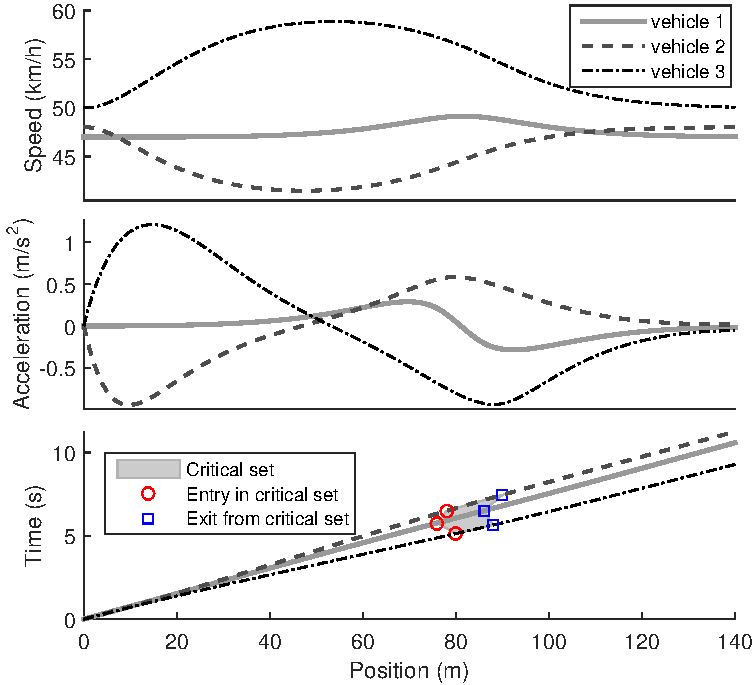
\includegraphics[width=\figwidth]{figures//trajectories}
\caption{Optimal state trajectories for an intersection scenario with three vehicles. The results depict the optimal crossing sequence \mbox{[3\; 1\; 2]}, where the subplots, from top to bottom, show the optimal speed, acceleration and travel time for each vehicle. The critical set, showing the position and time when each vehicle enters and exists the critical set, is depicted by the shaded region in the bottom plot.}
\label{fig:trajectories} %\vspace{-3.5mm}
\end{figure}

%%%%%%%%%%%%%%%%%%%%%%%%%%%%%%%%%%%%%%%%%%%%%%%%%%%%%%%%%%%%%%%%%%%%%%%%%%%%%%%
\section{Discussion and conclusion} \label{sec:conclusion}

This paper provides convex modeling steps for the problem of optimally controlling autonomous vehicles at intersections. For a chosen crossing sequence, we show that the remaining optimal control subproblem can be formulated as a convex program that can be efficiently solved. The method includes problem transformation from time to space domain and change of optimization variables, where vehicle speed is replaced by its inverse. We also provide simulation results showing the effectiveness of the proposed method.

Note that this paper proposes  a centralized control strategy. However, having shown that the optimal control subproblem is convex, it is possible to solve the control subproblem by distributed optimization \cite{boyd11}, where vehicles co-optimize their own objective in a parallel way.

The globally optimal solution of the original mixed-integer problem (\ref{eq:p1}), is obtained here by solving the optimal control subproblem (\ref{eq:p3}) for all possible permutations of crossing sequences. An obvious computational speedup with this approach would be to parallelize the computations over several processors, as the optimal control subproblems can be solved independently for the different crossing sequences. Another possibility is to solve the combined problem as a mixed-integer convex program, where branch and cut techniques can be used to reduce the number of crossing sequences that need to be investigated \cite{sager09}. Future research may include also the case where several vehicles travel on the same path, and where precedency constraints also need  be considered for safety enforcement.

%\vspace{-2mm}

\bibliographystyle{IEEEtran}
\bibliography{biblio,references}

\end{document}
